\section{Doxyblocks}\label{sec:doxyblocks}

DoxyBlocks is a plugin for \codeblocks that integrates doxygen into the IDE. It allows you to create documentation, insert comment blocks and run HTML or CHM documents. It also provides configuration of some of the more commonly used settings and access to doxywizard for more detailed configuration.

The settings in the DoxyBlocks toolbar have the following meanings:

\begin{description}
\item[
\includegraphics{Doxywizard}] Run doxywizard. Ctrl-Alt-D
\item[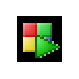
\includegraphics{Extract}] Extract documentation for the current project. Ctrl-Alt-E
\item[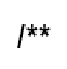
\includegraphics{Comment_block}] Insert a comment block at the current line. Additionally, DoxyBlocks will try to intelligently read if a method exists on the line for which a comment is being added. Ctrl-Alt-B

\begin{lstlisting}
/** \brief
 *
 * \param bar bool
 * \return void
 *
 */    
void MyClass::Foo(bool bar)
{
    fooBar(bar);
}
\end{lstlisting}

\item[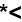
\includegraphics{Comment_line}] Insert a line comment at the current cursor position. Ctrl-Alt-L
\begin{lstlisting}
void MyClass::Foo(bool bar)
{
    fooBar(bar); /**<  */
}
\end{lstlisting}

\item[
\includegraphics{Html}] View generated HTML documentation. Ctrl-Alt-H
\item[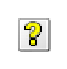
\includegraphics{Chm}] View generated HTML Help documentation. Ctrl-Alt-C
\item[
\includegraphics{Configure}] Open DoxyBlocks' preferences. Ctrl-Alt-P
\end{description}

Doxyblocks works only if doxygen is installed on your system. You need at least the executables doxygen and doxywizard (available in official doxygen distribution at \url{http://www.doxygen.nl/}). Optionally you can have the executable "dot" from the graphviz package (see \url{https://graphviz.gitlab.io/}. On Windows, the help compiler (hhc) may be used to generate chm files.

\genterm{Notes}
\begin{description}
\item In the preferences you have a check box to allow or not allow DoxyBlocks to \textbf{overwrite the doxyfile}. By default, if a doxyfile already exists it is not overwritten to protect any changes that have been made outside DoxyBlocks however this behaviour prevents changes made within DoxyBlocks being written to an existing doxyfile.
\item If a text field is blank in "Preferences", DoxyBlocks will assume that the corresponding executable is available somewhere in your environment's path. You can use macros such as \$(CODEBLOCKS) in your path and they will be expanded automatically.
\item [OUTPUT\_DIRECTORY] Used to specify the (relative or absolute) base path where the generated documentation will be put. If a relative path is entered, it will be relative to the location where doxygen was started. If left blank the current directory will be used. DoxyBlocks will use the path name entered here to create a directory relative to \codeline{<project dir>}. This allows you to create separate doxygen directories for projects that reside in the same directory, or just use a different directory name. If this field is blank, documents will be created in \codeline{<project dir>/doxygen}. Enter directory names without dots, leading separators, volume names, etc. DoxyBlocks does validation on the path name and will strip extraneous characters.
\begin{lstlisting}
Examples:
[blank]           -> <project dir>/doxygen.
"docs"            -> <project dir>/docs.
"docs/sub1/sub2"  -> <project dir>/docs/sub1/sub2.
"doxygen/docs"    -> <project dir>/doxygen/docs.
\end{lstlisting}
\item [OUTPUT\_LANGUAGE] Used to specify the language in which all documentation generated by doxygen is written. Doxygen will use this information to generate all constant output in the proper language. The default language is English. Other languages are supported. 
\item More information in doxygen help files
\end{description}